\section{Analyse technique}
	Cette section est destinée à préciser les détails d'implémentation des principales fonctionnalités présentées dans la section précédente. Cette section n'est pas complète car l'implémentation de certaines fonctionnalités n' a pas encore été étudiée.
	
	\subsection{Règles}
	%todo trouver un autre nom pour "target" qui suggère une entrée
	%todo mieux expliquer ce que désigne les champs d'une règle + exemple
		Les règles nécessaires au bon fonctionnement de notre générateur de contenu statique possèdent quatre champs obligatoires: \textit{Target}, \textit{Template}, \textit{Data} et \textit{Output}. Chacun de ces champs désigne un ou plusieurs fichiers grâce aux expressions régulières. La signification de chacun de ces quatre champs est expliquée ci-dessous. 
		
		\subsubsection*{Target}
			Les fichiers passés dans ce champs serviront de données pour le \textit{template}. Chaque fichier produira un fichier en sortie. C'est donc ce champ qui permet de gérer la multiplicité des fichiers de sortie.
		
		\subsubsection*{Template}
		%todo clarifier quel moteur de template gère le cas MultiTemplatesIn
			Ce champ désigne le fichier \textit{template} à utiliser sur les données chargées grâce aux champs \textit{Target} et \textit{Data}. 
			
			Concernant le cas \textit{MultiTemplatesIn} mentionné dans la Section 3, nous pouvons solutionner ce problème en utilisant l'héritage de \textit{template} de notre moteur de \textit{template}. Par défaut nous utiliserons le moteur \textit{Jinja2} \cite{Jinja2} qui supporte cette fonctionnalité. Le problème qui en découle est donc que ce cas d'utilisation ne sera réalisable que si on utilise un moteur de \textit{template} qui supporte une telle fonctionnalité.
			
			L'autre cas non-couvert, également exposé en Section 3, pouvant être solutionné est \textit{MultiTemplatesOut}. Dans l'état actuel des choses, il faudrait écrire la même règle \textbf{n} fois juste en changeant à chaque fois le champ \textit{template} par le fichier correspondant où \textbf{n} est le nombre de \textit{templates} à appliquer sur le fichier. Cette méthode deviendrait donc extrêmement lourde si le nombre de \textit{templates} à appliquer est important.
		
		\subsubsection*{Data}
			Les fichiers passés dans le champ \textit{Data} serviront également de données pour le \textit{template} comme \textit{Target}. La différence est que ce champ n'influence pas le nombre de fichiers de sortie. Les champs \textit{Target} et \textit{Data} permettent donc de gérer les multiplicités des fichiers d'entrée.
		
		\subsubsection*{Output}
			Ce champ permet de spécifier le nom des fichiers de sortie. L'utilisation de variables de champs mentionnées dans la Section 4 permettra par exemple de nommer chaque fichier de sortie en fonction de son "homonyme" passé au champ \textit{Target} ,et cela, peut importe la multiplicité en sortie.
	
	
	\subsection{Structure}
	%todo détailler et expliquer le diagramme de classe
		Comme mentionné dans la Section 4, nous appliquons la programmation modulaire afin de permettre une grande flexibilité à notre générateur de contenu statique. Nous avons donc conçu l'architecture dans cette optique comme le montre la Figure \ref{fig:class_diagram}. Un utilisateur pourra donc modifier le comportement de notre générateur en implémentant lui même l'une de ces interfaces. Il pourra, entre autres, modifier la syntaxe des règles mentionnées ci-dessus en implémentant l'interface \textit{RuleBackend}.
		
		Comme expliqué dans la section précédente, nous fournirons par défaut une implémentation de ces interfaces qui permettra à l'utilisateur de réaliser les cas d'utilisations listés en Section 2.
		
		\begin{figure}
			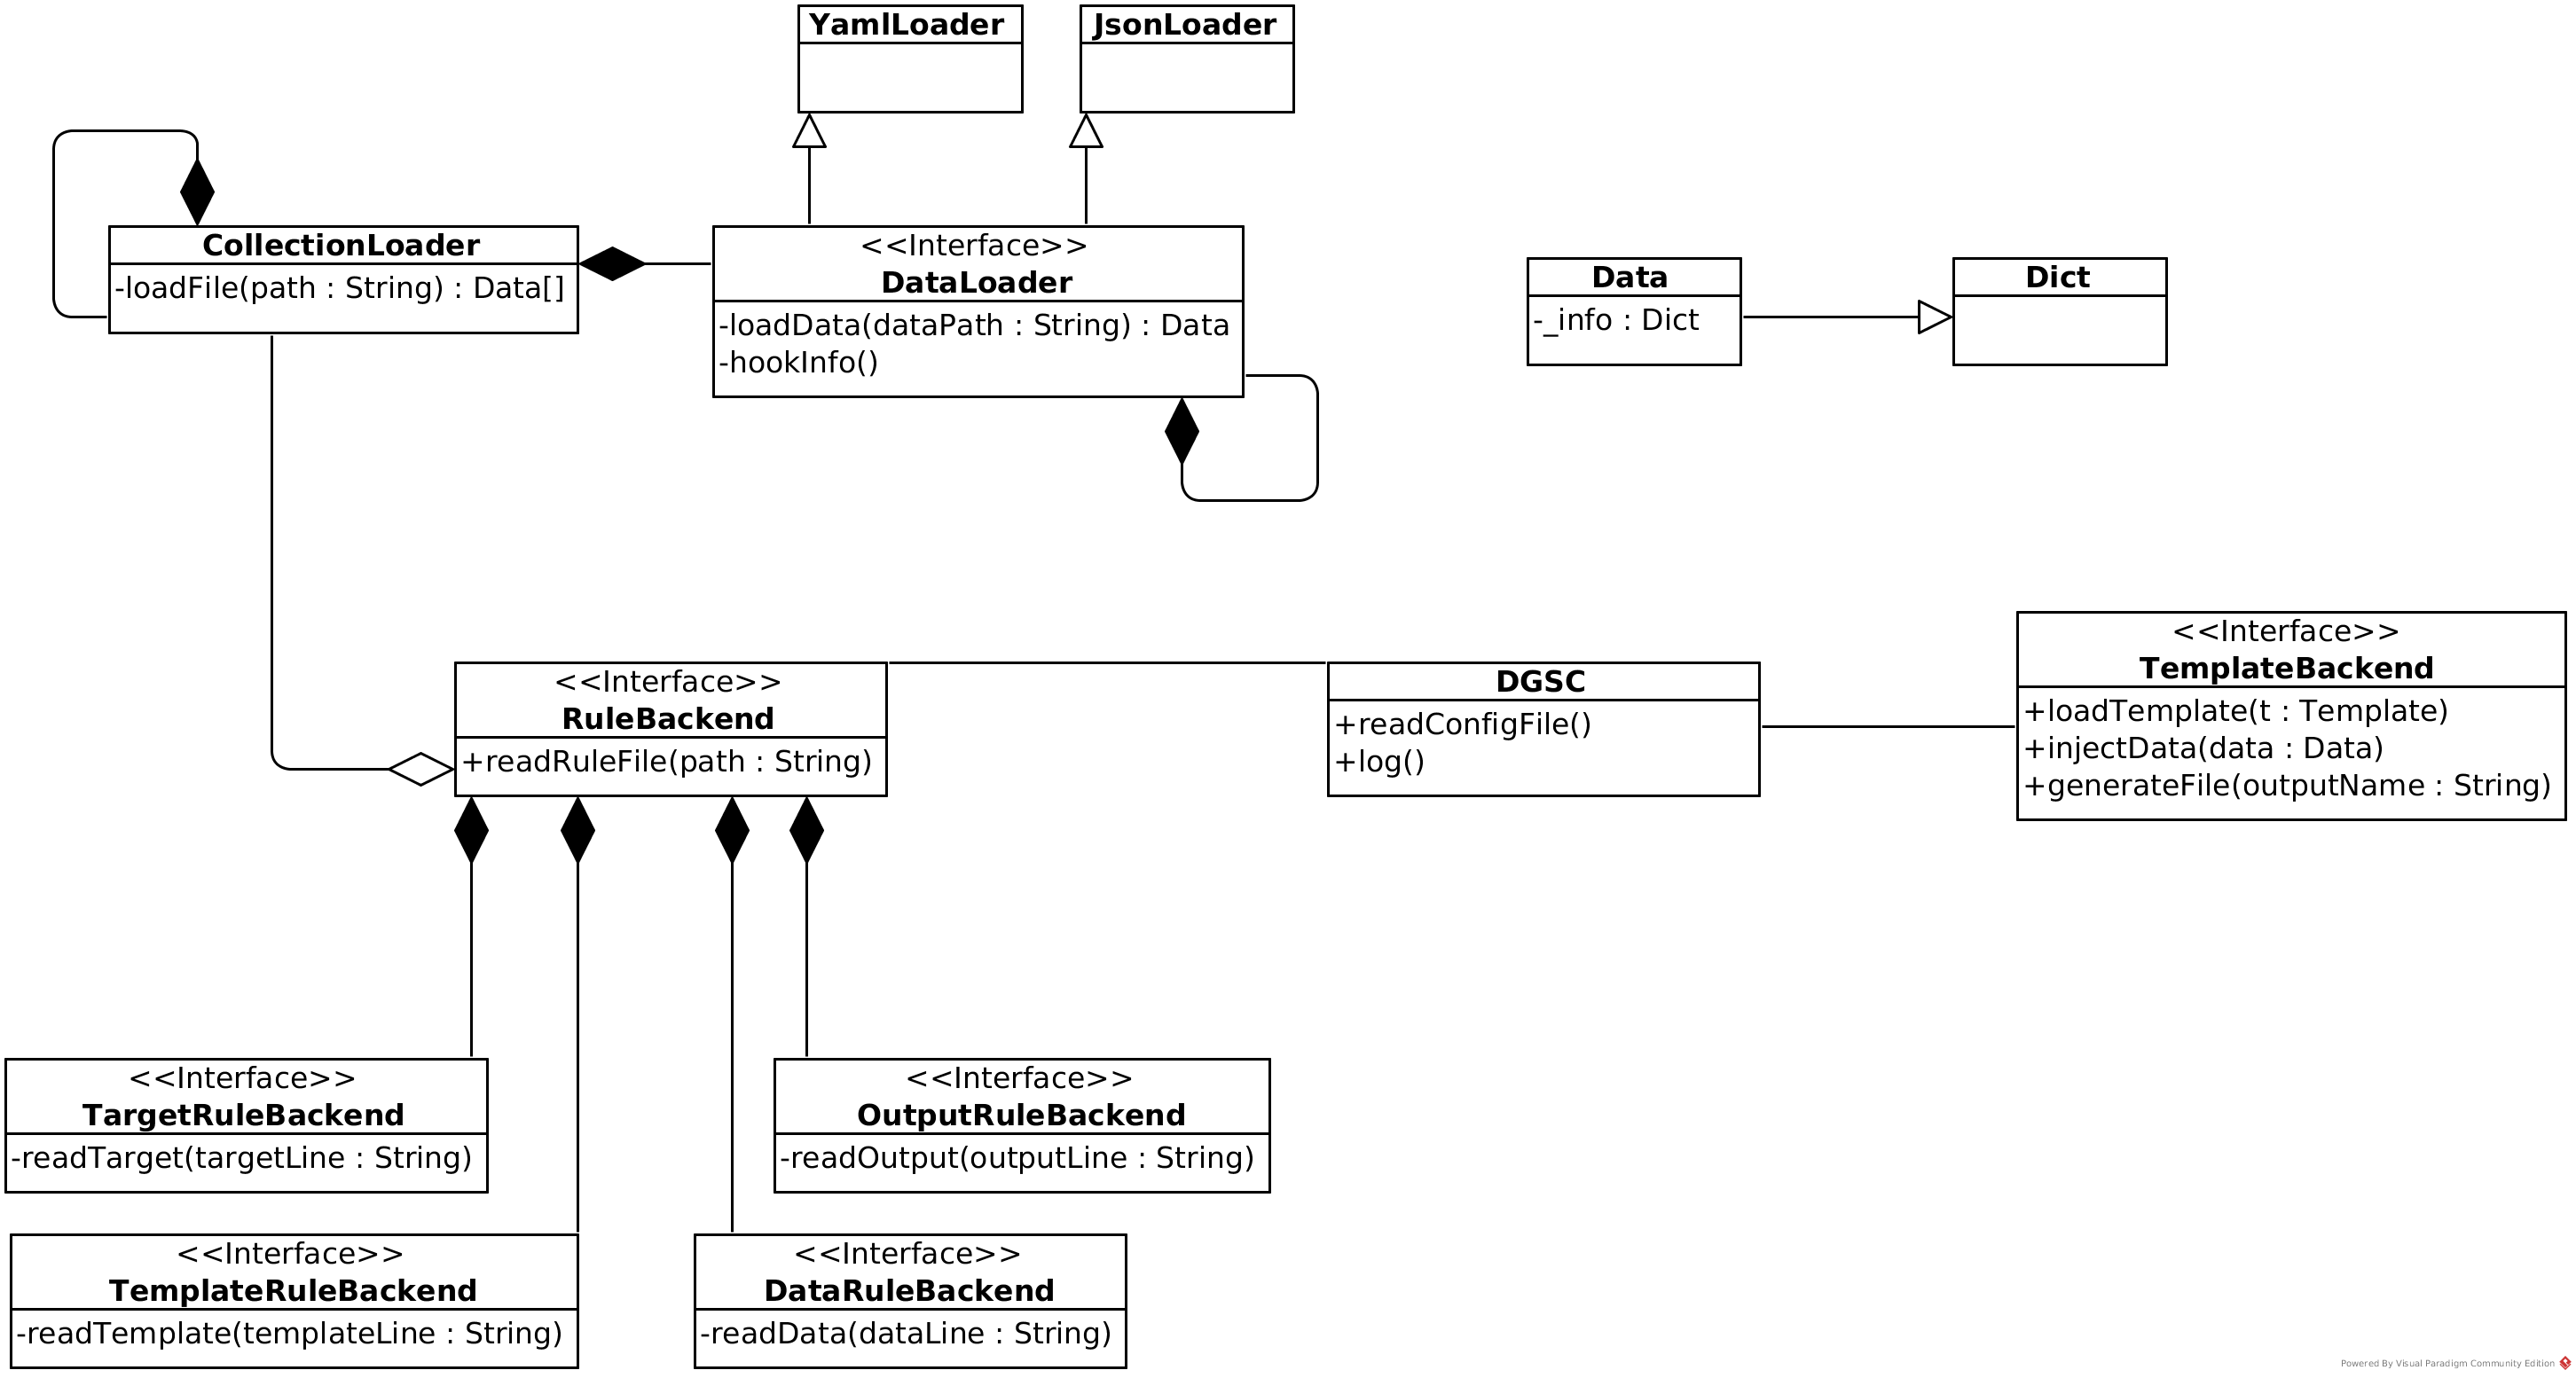
\includegraphics[width=\textwidth]{/diagrams/DGSC}
			\caption{Diagramme de classes de notre générateur de contenu statique}
			\label{fig:class_diagram}
		\end{figure} 
	
	
	\subsection{Configuration}
		Un fichier de configuration permettra à l'utilisateur de spécifier quelques options à notre générateur de contenu statique. Parmi ces options, nous retrouverons entre autres: le répertoire de travail en entrée, le répertoire de travail en sortie, une liste de classes implémentant les interfaces du générateur, l'emplacement du fichier de \textit{logs} (le cas échéant), ... Chacune de ses options aura une valeur par défaut, l'utilisateur ne devra donc spécifier que les éléments qui diffèrent de la configuration par défaut. 